\begin{frame}
    \frametitle{Material para Bundle Adjustment}
    \note{Extraído de Curso de Cyrill Stachniss https://youtu.be/LKDLcKrWOIU?si=InRBlf5Nmf7mGM9H}
    \begin{itemize}
        \item Cyrill Stachniss - The Basics about Bundle Adjustment Vídeo: \url{https://youtu.be/sobyKHwgB0Y?si=EqmuOjWNwKBI9jqH} Slides: \url{https://www.ipb.uni-bonn.de/html/teaching/photo12-2021/2021-pho2-09-BA-part1.pptx.pdf}
        \item Cyrill Stachniss - The Numerics of Bundle Adjustment Vídeo: \url{https://youtu.be/LKDLcKrWOIU?si=InRBlf5Nmf7mGM9H} Slides: \url{https://www.ipb.uni-bonn.de/html/teaching/photo12-2021/2021-pho2-10-BA-part2.pptx.pdf}
    \end{itemize}
\end{frame}

\begin{frame}
    \frametitle{Bundle Adjustment}
    \note{Información extraída de https://youtu.be/BuRCJ2fegcc y de https://youtu.be/mZBdPgBtrCM}
    
    \TODO{explicar mejor el hilo conductor de Levenberg–Marquardt a BA}
    
    Bundle Adjustment es un caso
    
    \begin{itemize}
        \item Reconstrucción 3D basada en imágenes tomadas de diferentes puntos de vista
        \item Minimiza el error de reproyección en el plano de la imagen 2D
        \item No hay noción de odometría (pose-pose constraints)
        \item En general utiliza como método de minimización Levenberg-Marquart
        \item Desarrollado en el área de Fotogrametría\footnote{Fotogrametría es la técnica cuyo objeto es estudiar y definir con precisión la forma, dimensiones y posición en el espacio de un objeto cualquiera, utilizando esencialmente medidas hechas sobre una o varias fotografías de ese objeto} durante la década de 1950
    \end{itemize}
    
\end{frame}

\begin{frame}
    \frametitle{Bundle Adjustment}
    
    \begin{figure}
        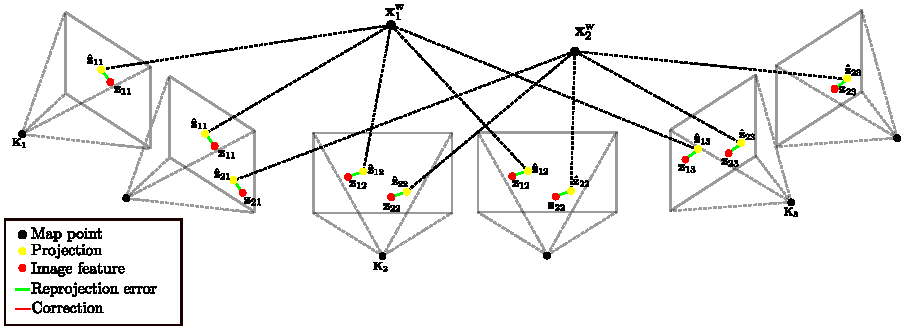
\includegraphics[width=\textwidth]{./images/ba_reprojection_error_before.pdf}
    \end{figure}
    
    \note{Ejemplo de ajuste de 3 keyframes que ven 2 puntos del mapa.\\
        k1 - x1 medición estéreo\\
        k1 - x2 medición derecha\\
        k2 - x1 medición estéreo\\
        k2 - x2 medición estéreo\\
        k3 - x1 medición izquierda\\
        k3 - x2 medición estéreo}
    
\end{frame}

\begin{frame}
    \frametitle{Bundle Adjustment}
    
    \begin{figure}
        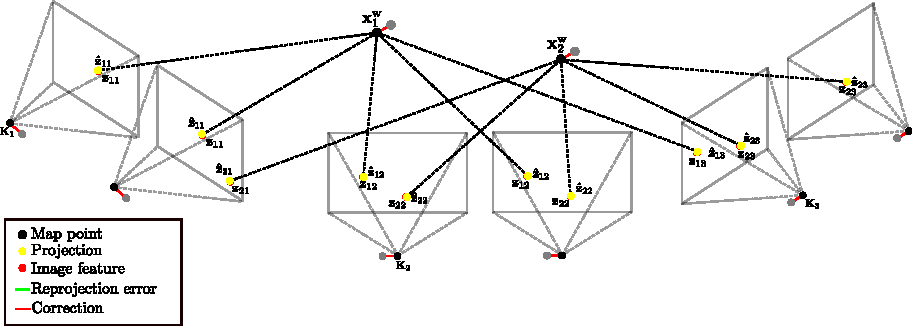
\includegraphics[width=\textwidth]{./images/ba_reprojection_error_after.pdf}
    \end{figure}
    
    \note{Ajustamos los keyframes y los puntos!!!\\
        Una ecuación de error por cada medición (6 en total).\\
        Nuevamente tenemos en cuenta la transformación rígida entre la cámara izquierda y la cámara derecha para las mediciones derechas.}
    
\end{frame}


\begin{frame}
    \frametitle{Bundle Adjustment}
    \note{Extraído de Cyrill Stachniss https://youtu.be/LKDLcKrWOIU?si=InRBlf5Nmf7mGM9H}
    
    Enfoque de mínimos cuadrados para estimar poses de cámara y puntos 3D
    
    \textbf{Idea Clave:}
    \begin{itemize}
        \item Comenzar con una solución inicial (\emph{inital guess})
        \item Proyectar los puntos 3D estimados en las imágenes de las cámaras estimadas
        \item Comparar ubicaciones de las proyecciones de los puntos 3D con los puntos medidos 2D
        \item Ajustar para minimizar el error en las imágenes.
    \end{itemize}
    
\end{frame}


